\def\schemaScenario simple_constraint_min{%
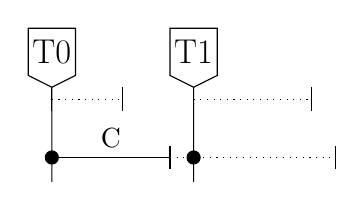
\begin{tikzpicture}[scale=0.3]%

\def\date{4};%
\def\nodeName{\Huge T0};%
\def\bottom{-10};%
\def\top{-6};%
\draw (\date,\top) -- ++(-1,0.5) -- ++(0,2) -- ++(2,0) -- ++(0,-2) -- ++(-1,-0.5) -- (\date, \bottom);%
\draw (\date,\top + 1.5) node[scale=0.5]{\nodeName};%
%
\def\date{10};%
\def\nodeName{\Huge T1};%
\def\bottom{-10};%
\def\top{-6};%
\draw (\date,\top) -- ++(-1,0.5) -- ++(0,2) -- ++(2,0) -- ++(0,-2) -- ++(-1,-0.5) -- (\date, \bottom);%
\draw (\date,\top + 1.5) node[scale=0.5]{\nodeName};%
%
\def\contraintName{C1};%
\def\ypos{-6.5};%
\def\date{0};
\def\min{4};%
\def\nom{6};%
\def\max{7};%
\draw (\date+\min,\ypos+0.5) -- ++(0,-1);%
\draw[dotted] (\date+\min,\ypos) -- (\date+\max,\ypos);%
\draw (\date+\max,\ypos+0.5) -- ++(0,-1);%
%
\def\contraintName{C};%
\def\ypos{-8.9719};%
\def\date{4};
\def\min{5};%
\def\nom{6};%
\def\max{12};%
\fill (\date,\ypos) circle (0.3);%
\fill (\date+\nom,\ypos) circle (0.3);%
\draw (\date,\ypos) -- ++(\min,0) node[midway,above,scale=1] {\contraintName};%
\draw (\date+\min,\ypos+0.5) -- ++(0,-1);%
\draw[dotted] (\date+\min,\ypos) -- (\date+\max,\ypos);%
\draw (\date+\max,\ypos+0.5) -- ++(0,-1);%
%
\def\contraintName{C3};%
\def\ypos{-6.5};%
\def\date{0};
\def\min{10};%
\def\nom{13};%
\def\max{15};%
\draw (\date+\min,\ypos+0.5) -- ++(0,-1);%
\draw[dotted] (\date+\min,\ypos) -- (\date+\max,\ypos);%
\draw (\date+\max,\ypos+0.5) -- ++(0,-1);%
%
\end{tikzpicture}%
}
